% Created by tikzDevice version 0.10.1 on 2016-09-01 14:16:45
% !TEX encoding = UTF-8 Unicode
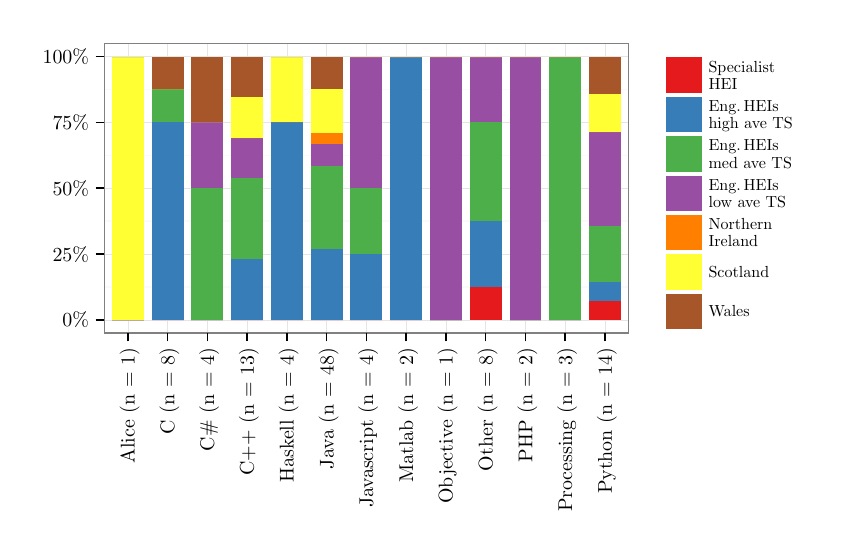
\begin{tikzpicture}[x=1pt,y=1pt]
\definecolor{fillColor}{RGB}{255,255,255}
\path[use as bounding box,fill=fillColor,fill opacity=0.00] (0,0) rectangle (289.08,180.67);
\begin{scope}
\path[clip] (  0.00,  0.00) rectangle (289.08,180.67);
\definecolor{drawColor}{RGB}{255,255,255}
\definecolor{fillColor}{RGB}{255,255,255}

\path[draw=drawColor,line width= 0.6pt,line join=round,line cap=round,fill=fillColor] (  0.00,  0.00) rectangle (289.08,180.68);
\end{scope}
\begin{scope}
\path[clip] ( 27.58, 70.28) rectangle (217.21,174.98);
\definecolor{fillColor}{RGB}{255,255,255}

\path[fill=fillColor] ( 27.58, 70.28) rectangle (217.21,174.98);
\definecolor{drawColor}{gray}{0.98}

\path[draw=drawColor,line width= 0.6pt,line join=round] ( 27.58, 86.93) --
	(217.21, 86.93);

\path[draw=drawColor,line width= 0.6pt,line join=round] ( 27.58,110.73) --
	(217.21,110.73);

\path[draw=drawColor,line width= 0.6pt,line join=round] ( 27.58,134.53) --
	(217.21,134.53);

\path[draw=drawColor,line width= 0.6pt,line join=round] ( 27.58,158.33) --
	(217.21,158.33);
\definecolor{drawColor}{gray}{0.90}

\path[draw=drawColor,line width= 0.2pt,line join=round] ( 27.58, 75.04) --
	(217.21, 75.04);

\path[draw=drawColor,line width= 0.2pt,line join=round] ( 27.58, 98.83) --
	(217.21, 98.83);

\path[draw=drawColor,line width= 0.2pt,line join=round] ( 27.58,122.63) --
	(217.21,122.63);

\path[draw=drawColor,line width= 0.2pt,line join=round] ( 27.58,146.43) --
	(217.21,146.43);

\path[draw=drawColor,line width= 0.2pt,line join=round] ( 27.58,170.22) --
	(217.21,170.22);

\path[draw=drawColor,line width= 0.2pt,line join=round] ( 36.20, 70.28) --
	( 36.20,174.98);

\path[draw=drawColor,line width= 0.2pt,line join=round] ( 50.56, 70.28) --
	( 50.56,174.98);

\path[draw=drawColor,line width= 0.2pt,line join=round] ( 64.93, 70.28) --
	( 64.93,174.98);

\path[draw=drawColor,line width= 0.2pt,line join=round] ( 79.30, 70.28) --
	( 79.30,174.98);

\path[draw=drawColor,line width= 0.2pt,line join=round] ( 93.66, 70.28) --
	( 93.66,174.98);

\path[draw=drawColor,line width= 0.2pt,line join=round] (108.03, 70.28) --
	(108.03,174.98);

\path[draw=drawColor,line width= 0.2pt,line join=round] (122.39, 70.28) --
	(122.39,174.98);

\path[draw=drawColor,line width= 0.2pt,line join=round] (136.76, 70.28) --
	(136.76,174.98);

\path[draw=drawColor,line width= 0.2pt,line join=round] (151.12, 70.28) --
	(151.12,174.98);

\path[draw=drawColor,line width= 0.2pt,line join=round] (165.49, 70.28) --
	(165.49,174.98);

\path[draw=drawColor,line width= 0.2pt,line join=round] (179.86, 70.28) --
	(179.86,174.98);

\path[draw=drawColor,line width= 0.2pt,line join=round] (194.22, 70.28) --
	(194.22,174.98);

\path[draw=drawColor,line width= 0.2pt,line join=round] (208.59, 70.28) --
	(208.59,174.98);
\definecolor{fillColor}{RGB}{228,26,28}

\path[fill=fillColor] ( 30.45, 75.04) rectangle ( 41.94, 75.04);
\definecolor{fillColor}{RGB}{55,126,184}

\path[fill=fillColor] ( 30.45, 75.04) rectangle ( 41.94, 75.04);
\definecolor{fillColor}{RGB}{77,175,74}

\path[fill=fillColor] ( 30.45, 75.04) rectangle ( 41.94, 75.04);
\definecolor{fillColor}{RGB}{152,78,163}

\path[fill=fillColor] ( 30.45, 75.04) rectangle ( 41.94, 75.04);
\definecolor{fillColor}{RGB}{255,127,0}

\path[fill=fillColor] ( 30.45, 75.04) rectangle ( 41.94, 75.04);
\definecolor{fillColor}{RGB}{255,255,51}

\path[fill=fillColor] ( 30.45, 75.04) rectangle ( 41.94,170.22);
\definecolor{fillColor}{RGB}{166,86,40}

\path[fill=fillColor] ( 30.45,170.22) rectangle ( 41.94,170.22);
\definecolor{fillColor}{RGB}{228,26,28}

\path[fill=fillColor] ( 44.82, 75.04) rectangle ( 56.31, 75.04);
\definecolor{fillColor}{RGB}{55,126,184}

\path[fill=fillColor] ( 44.82, 75.04) rectangle ( 56.31,146.43);
\definecolor{fillColor}{RGB}{77,175,74}

\path[fill=fillColor] ( 44.82,146.43) rectangle ( 56.31,158.33);
\definecolor{fillColor}{RGB}{152,78,163}

\path[fill=fillColor] ( 44.82,158.33) rectangle ( 56.31,158.33);
\definecolor{fillColor}{RGB}{255,127,0}

\path[fill=fillColor] ( 44.82,158.33) rectangle ( 56.31,158.33);
\definecolor{fillColor}{RGB}{255,255,51}

\path[fill=fillColor] ( 44.82,158.33) rectangle ( 56.31,158.33);
\definecolor{fillColor}{RGB}{166,86,40}

\path[fill=fillColor] ( 44.82,158.33) rectangle ( 56.31,170.22);
\definecolor{fillColor}{RGB}{228,26,28}

\path[fill=fillColor] ( 59.18, 75.04) rectangle ( 70.68, 75.04);
\definecolor{fillColor}{RGB}{55,126,184}

\path[fill=fillColor] ( 59.18, 75.04) rectangle ( 70.68, 75.04);
\definecolor{fillColor}{RGB}{77,175,74}

\path[fill=fillColor] ( 59.18, 75.04) rectangle ( 70.68,122.63);
\definecolor{fillColor}{RGB}{152,78,163}

\path[fill=fillColor] ( 59.18,122.63) rectangle ( 70.68,146.43);
\definecolor{fillColor}{RGB}{255,127,0}

\path[fill=fillColor] ( 59.18,146.43) rectangle ( 70.68,146.43);
\definecolor{fillColor}{RGB}{255,255,51}

\path[fill=fillColor] ( 59.18,146.43) rectangle ( 70.68,146.43);
\definecolor{fillColor}{RGB}{166,86,40}

\path[fill=fillColor] ( 59.18,146.43) rectangle ( 70.68,170.22);
\definecolor{fillColor}{RGB}{228,26,28}

\path[fill=fillColor] ( 73.55, 75.04) rectangle ( 85.04, 75.04);
\definecolor{fillColor}{RGB}{55,126,184}

\path[fill=fillColor] ( 73.55, 75.04) rectangle ( 85.04, 97.00);
\definecolor{fillColor}{RGB}{77,175,74}

\path[fill=fillColor] ( 73.55, 97.00) rectangle ( 85.04,126.29);
\definecolor{fillColor}{RGB}{152,78,163}

\path[fill=fillColor] ( 73.55,126.29) rectangle ( 85.04,140.94);
\definecolor{fillColor}{RGB}{255,127,0}

\path[fill=fillColor] ( 73.55,140.94) rectangle ( 85.04,140.94);
\definecolor{fillColor}{RGB}{255,255,51}

\path[fill=fillColor] ( 73.55,140.94) rectangle ( 85.04,155.58);
\definecolor{fillColor}{RGB}{166,86,40}

\path[fill=fillColor] ( 73.55,155.58) rectangle ( 85.04,170.22);
\definecolor{fillColor}{RGB}{228,26,28}

\path[fill=fillColor] ( 87.91, 75.04) rectangle ( 99.41, 75.04);
\definecolor{fillColor}{RGB}{55,126,184}

\path[fill=fillColor] ( 87.91, 75.04) rectangle ( 99.41,146.43);
\definecolor{fillColor}{RGB}{77,175,74}

\path[fill=fillColor] ( 87.91,146.43) rectangle ( 99.41,146.43);
\definecolor{fillColor}{RGB}{152,78,163}

\path[fill=fillColor] ( 87.91,146.43) rectangle ( 99.41,146.43);
\definecolor{fillColor}{RGB}{255,127,0}

\path[fill=fillColor] ( 87.91,146.43) rectangle ( 99.41,146.43);
\definecolor{fillColor}{RGB}{255,255,51}

\path[fill=fillColor] ( 87.91,146.43) rectangle ( 99.41,170.22);
\definecolor{fillColor}{RGB}{166,86,40}

\path[fill=fillColor] ( 87.91,170.22) rectangle ( 99.41,170.22);
\definecolor{fillColor}{RGB}{228,26,28}

\path[fill=fillColor] (102.28, 75.04) rectangle (113.77, 75.04);
\definecolor{fillColor}{RGB}{55,126,184}

\path[fill=fillColor] (102.28, 75.04) rectangle (113.77,100.82);
\definecolor{fillColor}{RGB}{77,175,74}

\path[fill=fillColor] (102.28,100.82) rectangle (113.77,130.56);
\definecolor{fillColor}{RGB}{152,78,163}

\path[fill=fillColor] (102.28,130.56) rectangle (113.77,138.50);
\definecolor{fillColor}{RGB}{255,127,0}

\path[fill=fillColor] (102.28,138.50) rectangle (113.77,142.46);
\definecolor{fillColor}{RGB}{255,255,51}

\path[fill=fillColor] (102.28,142.46) rectangle (113.77,158.33);
\definecolor{fillColor}{RGB}{166,86,40}

\path[fill=fillColor] (102.28,158.33) rectangle (113.77,170.22);
\definecolor{fillColor}{RGB}{228,26,28}

\path[fill=fillColor] (116.65, 75.04) rectangle (128.14, 75.04);
\definecolor{fillColor}{RGB}{55,126,184}

\path[fill=fillColor] (116.65, 75.04) rectangle (128.14, 98.83);
\definecolor{fillColor}{RGB}{77,175,74}

\path[fill=fillColor] (116.65, 98.83) rectangle (128.14,122.63);
\definecolor{fillColor}{RGB}{152,78,163}

\path[fill=fillColor] (116.65,122.63) rectangle (128.14,170.22);
\definecolor{fillColor}{RGB}{255,127,0}

\path[fill=fillColor] (116.65,170.22) rectangle (128.14,170.22);
\definecolor{fillColor}{RGB}{255,255,51}

\path[fill=fillColor] (116.65,170.22) rectangle (128.14,170.22);
\definecolor{fillColor}{RGB}{166,86,40}

\path[fill=fillColor] (116.65,170.22) rectangle (128.14,170.22);
\definecolor{fillColor}{RGB}{228,26,28}

\path[fill=fillColor] (131.01, 75.04) rectangle (142.50, 75.04);
\definecolor{fillColor}{RGB}{55,126,184}

\path[fill=fillColor] (131.01, 75.04) rectangle (142.50,170.22);
\definecolor{fillColor}{RGB}{77,175,74}

\path[fill=fillColor] (131.01,170.22) rectangle (142.50,170.22);
\definecolor{fillColor}{RGB}{152,78,163}

\path[fill=fillColor] (131.01,170.22) rectangle (142.50,170.22);
\definecolor{fillColor}{RGB}{255,127,0}

\path[fill=fillColor] (131.01,170.22) rectangle (142.50,170.22);
\definecolor{fillColor}{RGB}{255,255,51}

\path[fill=fillColor] (131.01,170.22) rectangle (142.50,170.22);
\definecolor{fillColor}{RGB}{166,86,40}

\path[fill=fillColor] (131.01,170.22) rectangle (142.50,170.22);
\definecolor{fillColor}{RGB}{228,26,28}

\path[fill=fillColor] (145.38, 75.04) rectangle (156.87, 75.04);
\definecolor{fillColor}{RGB}{55,126,184}

\path[fill=fillColor] (145.38, 75.04) rectangle (156.87, 75.04);
\definecolor{fillColor}{RGB}{77,175,74}

\path[fill=fillColor] (145.38, 75.04) rectangle (156.87, 75.04);
\definecolor{fillColor}{RGB}{152,78,163}

\path[fill=fillColor] (145.38, 75.04) rectangle (156.87,170.22);
\definecolor{fillColor}{RGB}{255,127,0}

\path[fill=fillColor] (145.38,170.22) rectangle (156.87,170.22);
\definecolor{fillColor}{RGB}{255,255,51}

\path[fill=fillColor] (145.38,170.22) rectangle (156.87,170.22);
\definecolor{fillColor}{RGB}{166,86,40}

\path[fill=fillColor] (145.38,170.22) rectangle (156.87,170.22);
\definecolor{fillColor}{RGB}{228,26,28}

\path[fill=fillColor] (159.74, 75.04) rectangle (171.24, 86.93);
\definecolor{fillColor}{RGB}{55,126,184}

\path[fill=fillColor] (159.74, 86.93) rectangle (171.24,110.73);
\definecolor{fillColor}{RGB}{77,175,74}

\path[fill=fillColor] (159.74,110.73) rectangle (171.24,146.43);
\definecolor{fillColor}{RGB}{152,78,163}

\path[fill=fillColor] (159.74,146.43) rectangle (171.24,170.22);
\definecolor{fillColor}{RGB}{255,127,0}

\path[fill=fillColor] (159.74,170.22) rectangle (171.24,170.22);
\definecolor{fillColor}{RGB}{255,255,51}

\path[fill=fillColor] (159.74,170.22) rectangle (171.24,170.22);
\definecolor{fillColor}{RGB}{166,86,40}

\path[fill=fillColor] (159.74,170.22) rectangle (171.24,170.22);
\definecolor{fillColor}{RGB}{228,26,28}

\path[fill=fillColor] (174.11, 75.04) rectangle (185.60, 75.04);
\definecolor{fillColor}{RGB}{55,126,184}

\path[fill=fillColor] (174.11, 75.04) rectangle (185.60, 75.04);
\definecolor{fillColor}{RGB}{77,175,74}

\path[fill=fillColor] (174.11, 75.04) rectangle (185.60, 75.04);
\definecolor{fillColor}{RGB}{152,78,163}

\path[fill=fillColor] (174.11, 75.04) rectangle (185.60,170.22);
\definecolor{fillColor}{RGB}{255,127,0}

\path[fill=fillColor] (174.11,170.22) rectangle (185.60,170.22);
\definecolor{fillColor}{RGB}{255,255,51}

\path[fill=fillColor] (174.11,170.22) rectangle (185.60,170.22);
\definecolor{fillColor}{RGB}{166,86,40}

\path[fill=fillColor] (174.11,170.22) rectangle (185.60,170.22);
\definecolor{fillColor}{RGB}{228,26,28}

\path[fill=fillColor] (188.48, 75.04) rectangle (199.97, 75.04);
\definecolor{fillColor}{RGB}{55,126,184}

\path[fill=fillColor] (188.48, 75.04) rectangle (199.97, 75.04);
\definecolor{fillColor}{RGB}{77,175,74}

\path[fill=fillColor] (188.48, 75.04) rectangle (199.97,170.22);
\definecolor{fillColor}{RGB}{152,78,163}

\path[fill=fillColor] (188.48,170.22) rectangle (199.97,170.22);
\definecolor{fillColor}{RGB}{255,127,0}

\path[fill=fillColor] (188.48,170.22) rectangle (199.97,170.22);
\definecolor{fillColor}{RGB}{255,255,51}

\path[fill=fillColor] (188.48,170.22) rectangle (199.97,170.22);
\definecolor{fillColor}{RGB}{166,86,40}

\path[fill=fillColor] (188.48,170.22) rectangle (199.97,170.22);
\definecolor{fillColor}{RGB}{228,26,28}

\path[fill=fillColor] (202.84, 75.04) rectangle (214.33, 81.83);
\definecolor{fillColor}{RGB}{55,126,184}

\path[fill=fillColor] (202.84, 81.83) rectangle (214.33, 88.63);
\definecolor{fillColor}{RGB}{77,175,74}

\path[fill=fillColor] (202.84, 88.63) rectangle (214.33,109.03);
\definecolor{fillColor}{RGB}{152,78,163}

\path[fill=fillColor] (202.84,109.03) rectangle (214.33,143.03);
\definecolor{fillColor}{RGB}{255,127,0}

\path[fill=fillColor] (202.84,143.03) rectangle (214.33,143.03);
\definecolor{fillColor}{RGB}{255,255,51}

\path[fill=fillColor] (202.84,143.03) rectangle (214.33,156.63);
\definecolor{fillColor}{RGB}{166,86,40}

\path[fill=fillColor] (202.84,156.63) rectangle (214.33,170.22);
\definecolor{drawColor}{gray}{0.50}

\path[draw=drawColor,line width= 0.6pt,line join=round,line cap=round] ( 27.58, 70.28) rectangle (217.21,174.98);
\end{scope}
\begin{scope}
\path[clip] (  0.00,  0.00) rectangle (289.08,180.67);
\definecolor{drawColor}{RGB}{0,0,0}

\node[text=drawColor,anchor=base east,inner sep=0pt, outer sep=0pt, scale=  0.72] at ( 22.18, 72.56) {0\%};

\node[text=drawColor,anchor=base east,inner sep=0pt, outer sep=0pt, scale=  0.72] at ( 22.18, 96.35) {25\%};

\node[text=drawColor,anchor=base east,inner sep=0pt, outer sep=0pt, scale=  0.72] at ( 22.18,120.15) {50\%};

\node[text=drawColor,anchor=base east,inner sep=0pt, outer sep=0pt, scale=  0.72] at ( 22.18,143.95) {75\%};

\node[text=drawColor,anchor=base east,inner sep=0pt, outer sep=0pt, scale=  0.72] at ( 22.18,167.75) {100\%};
\end{scope}
\begin{scope}
\path[clip] (  0.00,  0.00) rectangle (289.08,180.67);
\definecolor{drawColor}{RGB}{0,0,0}

\path[draw=drawColor,line width= 0.6pt,line join=round] ( 24.58, 75.04) --
	( 27.58, 75.04);

\path[draw=drawColor,line width= 0.6pt,line join=round] ( 24.58, 98.83) --
	( 27.58, 98.83);

\path[draw=drawColor,line width= 0.6pt,line join=round] ( 24.58,122.63) --
	( 27.58,122.63);

\path[draw=drawColor,line width= 0.6pt,line join=round] ( 24.58,146.43) --
	( 27.58,146.43);

\path[draw=drawColor,line width= 0.6pt,line join=round] ( 24.58,170.22) --
	( 27.58,170.22);
\end{scope}
\begin{scope}
\path[clip] (  0.00,  0.00) rectangle (289.08,180.67);
\definecolor{drawColor}{RGB}{0,0,0}

\path[draw=drawColor,line width= 0.6pt,line join=round] ( 36.20, 67.28) --
	( 36.20, 70.28);

\path[draw=drawColor,line width= 0.6pt,line join=round] ( 50.56, 67.28) --
	( 50.56, 70.28);

\path[draw=drawColor,line width= 0.6pt,line join=round] ( 64.93, 67.28) --
	( 64.93, 70.28);

\path[draw=drawColor,line width= 0.6pt,line join=round] ( 79.30, 67.28) --
	( 79.30, 70.28);

\path[draw=drawColor,line width= 0.6pt,line join=round] ( 93.66, 67.28) --
	( 93.66, 70.28);

\path[draw=drawColor,line width= 0.6pt,line join=round] (108.03, 67.28) --
	(108.03, 70.28);

\path[draw=drawColor,line width= 0.6pt,line join=round] (122.39, 67.28) --
	(122.39, 70.28);

\path[draw=drawColor,line width= 0.6pt,line join=round] (136.76, 67.28) --
	(136.76, 70.28);

\path[draw=drawColor,line width= 0.6pt,line join=round] (151.12, 67.28) --
	(151.12, 70.28);

\path[draw=drawColor,line width= 0.6pt,line join=round] (165.49, 67.28) --
	(165.49, 70.28);

\path[draw=drawColor,line width= 0.6pt,line join=round] (179.86, 67.28) --
	(179.86, 70.28);

\path[draw=drawColor,line width= 0.6pt,line join=round] (194.22, 67.28) --
	(194.22, 70.28);

\path[draw=drawColor,line width= 0.6pt,line join=round] (208.59, 67.28) --
	(208.59, 70.28);
\end{scope}
\begin{scope}
\path[clip] (  0.00,  0.00) rectangle (289.08,180.67);
\definecolor{drawColor}{RGB}{0,0,0}

\node[text=drawColor,rotate= 90.00,anchor=base east,inner sep=0pt, outer sep=0pt, scale=  0.72] at ( 38.68, 64.88) {Alice (n = 1)};

\node[text=drawColor,rotate= 90.00,anchor=base east,inner sep=0pt, outer sep=0pt, scale=  0.72] at ( 53.04, 64.88) {C (n = 8)};

\node[text=drawColor,rotate= 90.00,anchor=base east,inner sep=0pt, outer sep=0pt, scale=  0.72] at ( 67.41, 64.88) {C\# (n = 4)};

\node[text=drawColor,rotate= 90.00,anchor=base east,inner sep=0pt, outer sep=0pt, scale=  0.72] at ( 81.77, 64.88) {C++ (n = 13)};

\node[text=drawColor,rotate= 90.00,anchor=base east,inner sep=0pt, outer sep=0pt, scale=  0.72] at ( 96.14, 64.88) {Haskell (n = 4)};

\node[text=drawColor,rotate= 90.00,anchor=base east,inner sep=0pt, outer sep=0pt, scale=  0.72] at (110.51, 64.88) {Java (n = 48)};

\node[text=drawColor,rotate= 90.00,anchor=base east,inner sep=0pt, outer sep=0pt, scale=  0.72] at (124.87, 64.88) {Javascript (n = 4)};

\node[text=drawColor,rotate= 90.00,anchor=base east,inner sep=0pt, outer sep=0pt, scale=  0.72] at (139.24, 64.88) {Matlab (n = 2)};

\node[text=drawColor,rotate= 90.00,anchor=base east,inner sep=0pt, outer sep=0pt, scale=  0.72] at (153.60, 64.88) {Objective (n = 1)};

\node[text=drawColor,rotate= 90.00,anchor=base east,inner sep=0pt, outer sep=0pt, scale=  0.72] at (167.97, 64.88) {Other (n = 8)};

\node[text=drawColor,rotate= 90.00,anchor=base east,inner sep=0pt, outer sep=0pt, scale=  0.72] at (182.33, 64.88) {PHP (n = 2)};

\node[text=drawColor,rotate= 90.00,anchor=base east,inner sep=0pt, outer sep=0pt, scale=  0.72] at (196.70, 64.88) {Processing (n = 3)};

\node[text=drawColor,rotate= 90.00,anchor=base east,inner sep=0pt, outer sep=0pt, scale=  0.72] at (211.07, 64.88) {Python (n = 14)};
\end{scope}
\begin{scope}
\path[clip] (  0.00,  0.00) rectangle (289.08,180.67);
\definecolor{fillColor}{RGB}{255,255,255}

\path[fill=fillColor] (225.74, 66.76) rectangle (280.54,178.50);
\end{scope}
\begin{scope}
\path[clip] (  0.00,  0.00) rectangle (289.08,180.67);
\definecolor{fillColor}{RGB}{228,26,28}

\path[fill=fillColor] (230.72,157.10) rectangle (243.53,169.90);
\end{scope}
\begin{scope}
\path[clip] (  0.00,  0.00) rectangle (289.08,180.67);
\definecolor{fillColor}{RGB}{55,126,184}

\path[fill=fillColor] (230.72,142.87) rectangle (243.53,155.68);
\end{scope}
\begin{scope}
\path[clip] (  0.00,  0.00) rectangle (289.08,180.67);
\definecolor{fillColor}{RGB}{77,175,74}

\path[fill=fillColor] (230.72,128.65) rectangle (243.53,141.45);
\end{scope}
\begin{scope}
\path[clip] (  0.00,  0.00) rectangle (289.08,180.67);
\definecolor{fillColor}{RGB}{152,78,163}

\path[fill=fillColor] (230.72,114.42) rectangle (243.53,127.23);
\end{scope}
\begin{scope}
\path[clip] (  0.00,  0.00) rectangle (289.08,180.67);
\definecolor{fillColor}{RGB}{255,127,0}

\path[fill=fillColor] (230.72,100.20) rectangle (243.53,113.00);
\end{scope}
\begin{scope}
\path[clip] (  0.00,  0.00) rectangle (289.08,180.67);
\definecolor{fillColor}{RGB}{255,255,51}

\path[fill=fillColor] (230.72, 85.97) rectangle (243.53, 98.77);
\end{scope}
\begin{scope}
\path[clip] (  0.00,  0.00) rectangle (289.08,180.67);
\definecolor{fillColor}{RGB}{166,86,40}

\path[fill=fillColor] (230.72, 71.74) rectangle (243.53, 84.55);
\end{scope}
\begin{scope}
\path[clip] (  0.00,  0.00) rectangle (289.08,180.67);
\definecolor{drawColor}{RGB}{0,0,0}

\node[text=drawColor,anchor=base west,inner sep=0pt, outer sep=0pt, scale=  0.58] at (246.04,164.63) {Specialist};

\node[text=drawColor,anchor=base west,inner sep=0pt, outer sep=0pt, scale=  0.58] at (246.04,158.41) {HEI};
\end{scope}
\begin{scope}
\path[clip] (  0.00,  0.00) rectangle (289.08,180.67);
\definecolor{drawColor}{RGB}{0,0,0}

\node[text=drawColor,anchor=base west,inner sep=0pt, outer sep=0pt, scale=  0.58] at (246.04,150.40) {Eng.\,HEIs};

\node[text=drawColor,anchor=base west,inner sep=0pt, outer sep=0pt, scale=  0.58] at (246.04,144.18) {high ave TS};
\end{scope}
\begin{scope}
\path[clip] (  0.00,  0.00) rectangle (289.08,180.67);
\definecolor{drawColor}{RGB}{0,0,0}

\node[text=drawColor,anchor=base west,inner sep=0pt, outer sep=0pt, scale=  0.58] at (246.04,136.18) {Eng.\,HEIs};

\node[text=drawColor,anchor=base west,inner sep=0pt, outer sep=0pt, scale=  0.58] at (246.04,129.96) {med ave TS};
\end{scope}
\begin{scope}
\path[clip] (  0.00,  0.00) rectangle (289.08,180.67);
\definecolor{drawColor}{RGB}{0,0,0}

\node[text=drawColor,anchor=base west,inner sep=0pt, outer sep=0pt, scale=  0.58] at (246.04,121.95) {Eng.\,HEIs};

\node[text=drawColor,anchor=base west,inner sep=0pt, outer sep=0pt, scale=  0.58] at (246.04,115.73) {low ave TS};
\end{scope}
\begin{scope}
\path[clip] (  0.00,  0.00) rectangle (289.08,180.67);
\definecolor{drawColor}{RGB}{0,0,0}

\node[text=drawColor,anchor=base west,inner sep=0pt, outer sep=0pt, scale=  0.58] at (246.04,107.72) {Northern};

\node[text=drawColor,anchor=base west,inner sep=0pt, outer sep=0pt, scale=  0.58] at (246.04,101.50) {Ireland};
\end{scope}
\begin{scope}
\path[clip] (  0.00,  0.00) rectangle (289.08,180.67);
\definecolor{drawColor}{RGB}{0,0,0}

\node[text=drawColor,anchor=base west,inner sep=0pt, outer sep=0pt, scale=  0.58] at (246.04, 90.39) {Scotland};
\end{scope}
\begin{scope}
\path[clip] (  0.00,  0.00) rectangle (289.08,180.67);
\definecolor{drawColor}{RGB}{0,0,0}

\node[text=drawColor,anchor=base west,inner sep=0pt, outer sep=0pt, scale=  0.58] at (246.04, 76.16) {Wales};
\end{scope}
\end{tikzpicture}
